% !TEX root = ../Masters.tex
\chapter{Evaluation of DGEL}
DGEL consists of to main modules: \textit{generation} and \textit{evaluation}.
The evaluation module consists of the fitness component which evaluates who good the L-system plants are.
The remaining components are part of the generation component which generates plants, and uses the evaluation module to generate \textit{good} plants.
To answer if DGEL solves the research questions, both modules have to be evaluated.
The generation module will be evaluated in a technical manner to determine if it performs well or not.
The evaluation module will be evaluated using humans as to answer if the fitness function properly rates plants as aesthetically pleasing or not.

\section{Evaluation of the Generation Module}
\subsection{Method}
As explained in Section~\ref{sec:overview} and shown in Figure~\ref{fig:dgel}, there are two main processes involved in generating the model for the L-system plants: \textit{SA} and \textit{GE}.
The remaining steps are dependent on the model and do not create variations on the same model.
Thus GE and SA are the two processes of interests to evaluate.

% GE SA vs GE uniform - need data, how to measure?

\subsubsection{Grammar Evolution}
GE, as with GA, depends on multiple parameter, and with tournament sampling there are even more.
Thus, before evaluation the GE process, good parameters had to be found.
Additionally, seeing what parameters are needed for a good performing GE may reveal additional properties of it.
The parameters were found using a combined manual and automated approach by searching the parameter space in multiple steps.
The idea was not to find the optimal parameters, but rather to find some parameters that made the GE produce an individual with good fitness within a reasonable time.
It was assumed that the size parameters -- population size and number of generations -- are the baseline parameters for GE and thus should be found first.
Then the tournament size for the tournament selection strategy should be found.
Then good parameters for the recombination rates -- crossover rate and mutation rate -- should be found.
Finally the parameter for the GE gene duplication operator should be found.

To search for the GE parameters, a breadth-first graph search inspired approach was used.
An example is shown in Figure~\ref{fig:parameter-search}.
The approach tests a combination of parameters by doing 20 GE runs with those parameters and using the mean fitness score of the best individual from each run.
If the score is an improvement of the previous score, the search will also tests the neighboring nodes in the graph by increasing the parameter values.
Otherwise, the current parameter values will be considered as not improving the performance and thus be discarded.
When there are no more improvements, the parameter values that produced the best score will be returned.
The parameter values will start at a small value and increase in an exponential fashion.
This is based on the assumption that the parameters are more sensitive when the values are small.
All of the parameter searches, except for the reproduction parameter search, will increase with a multiplicative of 2.
Because the reproduction rate parameters are bounded ($[0, 1]$) and to cover the whole range with a reasonable amount of steps, custom steps of 0.01, 0.1, 0.5 and 1 were used.

\begin{figure}
    \centering
    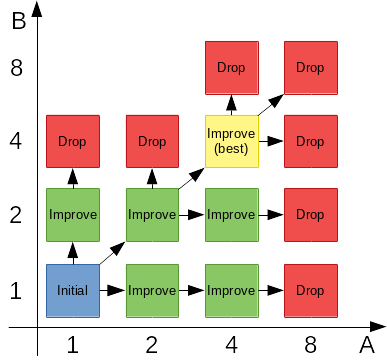
\includegraphics[width=0.6\textwidth]{figures/parameter-search}
    \caption{Example of a GE parameter search}
    \label{fig:parameter-search}
\end{figure}

% Formulate this as a hypothesis?
To evaluate the GE process, it was compared to completely random set of L-systems.
If the best individual from the GE process has a higher fitness score than the best individual from the random set of individuals, the GE process is an improvement.
To make a fair comparison, the random set of individuals should contain as many individuals as the GE generates and modifies (through mutation or crossover)
This way, both methods will ``generate'' the same amount of individuals, either being completely new individuals or modifications of existing individuals.
GE uses a fixed number of generations and population size, resulting into a fixed number of chromosome generations and modifications: $individuals = population + population * generations$.
Thus the random set method will generate $individuals$ individuals.

Because both methods depend on a random seed, an average of multiple runs will have to be used.
A sample size of 11 was selected as balanced choice between sample size and duration.
Student's t-test was used to test the group mean difference.

\subsubsection{Simulated Annealing}
To evaluate the SA process, a list of questions were made:
\begin{itemize}
	\item Can SA and the grammar distribution be used to find portions of the parameter space that generate better L-system plants?
	\item Does SA enable GE to find better L-system plants?
	\item Can SA find multiple portions of the parameter space that each generate unique-looking plants?
\end{itemize}
To answer the first question, two methods were used.
First, SA was used as described in previous sections to find an optimized grammar distribution, and the progress of it was plotted.
The progress plot was analyzed to see if SA made any meaningful progress.
Secondly, a comparison was made between the average fitness of L-systems randomly generated by a uniform grammar distribution and L-systems randomly generated by an SA-optimized grammar distribution.
The L-systems were generated in a completely random manner, not using any evolutionary approach such as GE.
% I need to actually run this experiment....
While this may answer if it is possible for an SA-optimized grammar distribution to generate better plants, it does not answer if this always will be the case.

To answer the second question, the performance of GE with a uniform grammar distribution was compared to the performance of GE with an SA-optimized grammar distribution.
Both GE processes were run 11 times, each time extracting the best L-system, before taking the mean of the best L-systems and using a t-test to test if the means were different.

\subsection{Results}
\subsubsection{Grammar Evolution}
Figure~\ref{fig:size-sampling} shows the search of the population size and number of generations to be used for the GE process.
The search was prematurely stopped because at around either 1600 number of generations or population size the duration became unreasonable long.
As seen, a minimum of either a population size of 200 or 200 generations is required for a reasonable performance.
Additionally, for any number of generations, a population size of 200 makes a notable improvement.
From this point, there is a steady improvement from around 0.8 to 0.9 with both parameters increasing towards 1600.
Outside a line drawn through 800, 400 and 400, 800 there does not seem to be any notable improvement, while the duration increases by a large amount.
The parameter values that yielded the best fitness was $generations = 200$ and $population size = 800$, and they did it within a reasonable duration.
The duration of it is significantly smaller than other parameter values that yield approximately the same fitness.
Thus, these parameter values were selected for use.

\begin{figure}
    \centering
    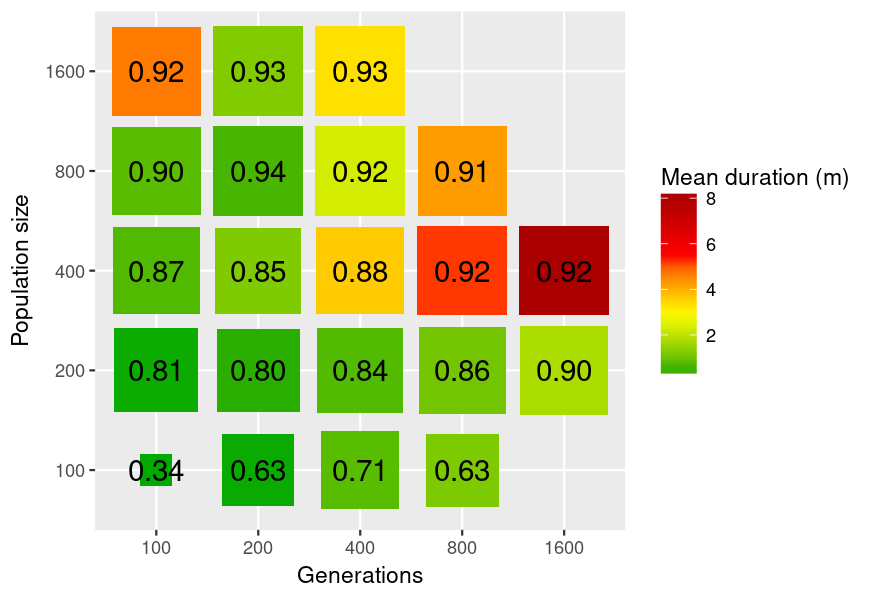
\includegraphics[width=0.8\textwidth]{figures/ge-size-sampling}
    \caption[Visualized search of GE population size and number of generations]{Visualized search of GE population size and number of generations. Numbers are the mean of best fitness scores, box sizes are a representation of that number, and colors represent the mean duration of the GE.}
    \label{fig:size-sampling}
\end{figure}

Figure~\ref{fig:tournament-sampling} shows the search of the tournament size.
Contrasted to the other searches, this is a one-dimensional search.
% Possibly do a significance test. Need to re-run to generate raw data...
As seen in the figure, the search did not find any improvements at all.
% A BIG LIMITATION IS THAT A LARGER TOURNAMENT SIZE MAY ENABLE SMALLER SIZE PARAMETERS.
Thus the tournament size was kept at the lowest value, i.e.\ 2.

\begin{figure}
    \centering
    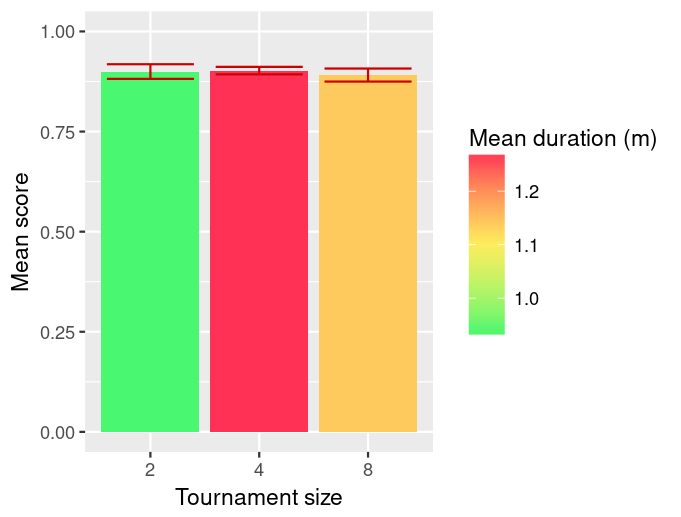
\includegraphics[width=0.7\textwidth]{figures/ge-tournament-sampling}
    \caption{Visualized search of the GE tournament selection tournament size}
    \label{fig:tournament-sampling}
\end{figure}

Figure~\ref{fig:recombination-sampling} shows the search of the recombination parameters: mutation rate and crossover rate.
There is a general improvement in fitness with both increasing mutation rate and crossover rate until the crossover rate reaches 1 where it suddenly turns for the worse.
Thus the crossover rate should at least be below 1.
Additionally, the crossover rate seems to be the parameter that contributes less to an improved fitness and increases the duration the most.
Thus the mutation rate should be the most important parameter.
The best fitness score is provided by a mutation rate of 1 and crossover rate of 0.5, further indicating this.

Figure~\ref{fig:recombination-sampling-variance} Shows the same standard deviations in the same search.
The pattern is similar to that of the mean fitness scores.
The most stable performance is provided by a mutation rate of 1 and crossover rate of 0.5.
Thus the recombination parameters will be using these values.

\begin{figure}
    \centering
    \begin{subfigure}{0.57\textwidth}
        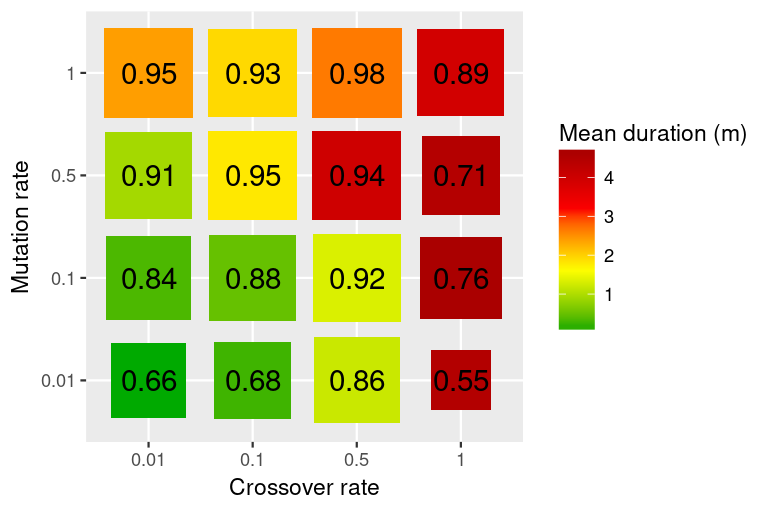
\includegraphics[width=\textwidth]{figures/ge-recombination-sampling}
        \caption{Mean of best fitness scores as numbers and sizes, with duration as colors}
        \label{fig:recombination-sampling}
    \end{subfigure}
    ~
    \begin{subfigure}{0.4\textwidth}
        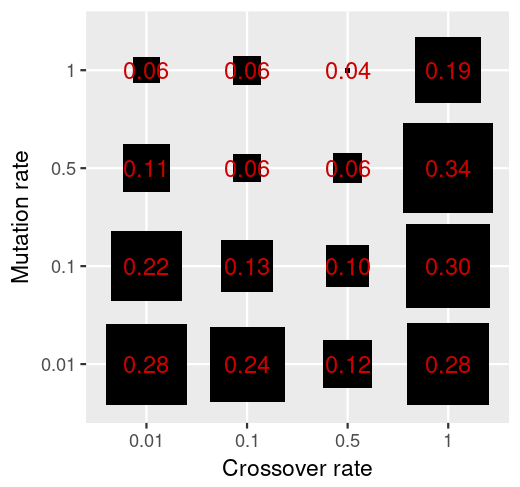
\includegraphics[width=\textwidth]{figures/ge-recombination-sampling-variance}
        \caption{Standard deviation}
        \label{fig:recombination-sampling-variance}
    \end{subfigure}
    \caption{Visualized search of the GE recombination parameters}
\end{figure}

% WHAT ABOUT DUPLICATION RATE
All of the GE parameters are summarized in Table~\ref{tab:ge-parameters}.

\begin{table}
    \centering
    \begin{tabular}{| l | l |}
    \hline
    \textbf{Parameter} & \textbf{Value} \\ \hline
    Population size & 800 \\
    \hline
    Generations & 200 \\
    \hline
    Tournament size & 2 \\
    \hline
    Mutation rate & 1.0 \\
    \hline
    Crossover rate & 0.5 \\
    \hline
    Duplication rate & 0 \\
    \hline
    \end{tabular}
    \caption{GE parameter values selected based on searches}
    \label{tab:ge-parameters}
\end{table}

Figure~\ref{fig:ge-random} shows the comparison of GE against random samples.
The difference in mean of best fitness is 0.13 (p < 0.01), where GE has a higher mean than random.
Thus there is a statistically significant difference between their performances.
Additionally, Figure~\ref{fig:ge-random-duration} shows the mean duration of the methods where GE is 5 times faster than random.
This indicates that GE is indeed an improvement of randomly generating samples.

\begin{figure}
    \centering
    \begin{subfigure}{0.4\textwidth}
        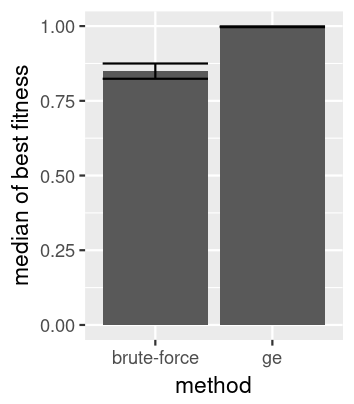
\includegraphics[width=\textwidth]{figures/ge-random}
        \caption{Mean of best fitness}
        \label{fig:ge-random}
    \end{subfigure}
    ~
    \begin{subfigure}{0.4\textwidth}
        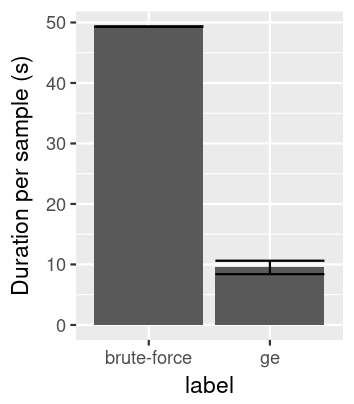
\includegraphics[width=\textwidth]{figures/ge-random-duration}
        \caption{Mean duration}
        \label{fig:ge-random-duration}
    \end{subfigure}
    \caption{GE and random performance compared}
\end{figure}

\subsubsection{Simulated Annealing}

Figure~\ref{fig:sa-progress} shows the progress of one SA run, and Figure~\ref{fig:sa-progress-close} shows a close-up of the first annealing.
The run had a maximum of 2000 moves per dimension and a cooldown rate of 0.002.
The grammar distribution evaluation had a minimum 32 samples and an error threshold of 0.004.
In total this resulted into 436000 moves over 9 annealings.
As seen in the figure, for each annealing there is a general improvement from a fitness score of 0 to around 0.6.
As expected, the SA process explores the space in the beginning, moving both up and down in score, and then gradually focuses more on hill climbing towards the end.
Each annealing generally reach a plateau before being halfway through the annealing process, from when nearly all mutations are worse and thus it chooses to stay, though the second annealing is slower to reach the plateau.
The fourth annealing found one exceptionally good grammar distribution with a score of almost 0.75, but when the same grammar distribution was measured over 100000 samples its score was 0.61, as seen in Figure~\ref{fig:sa-uniform}.
Thus the score measured in the SA process may have been inaccurate.

\begin{figure}
    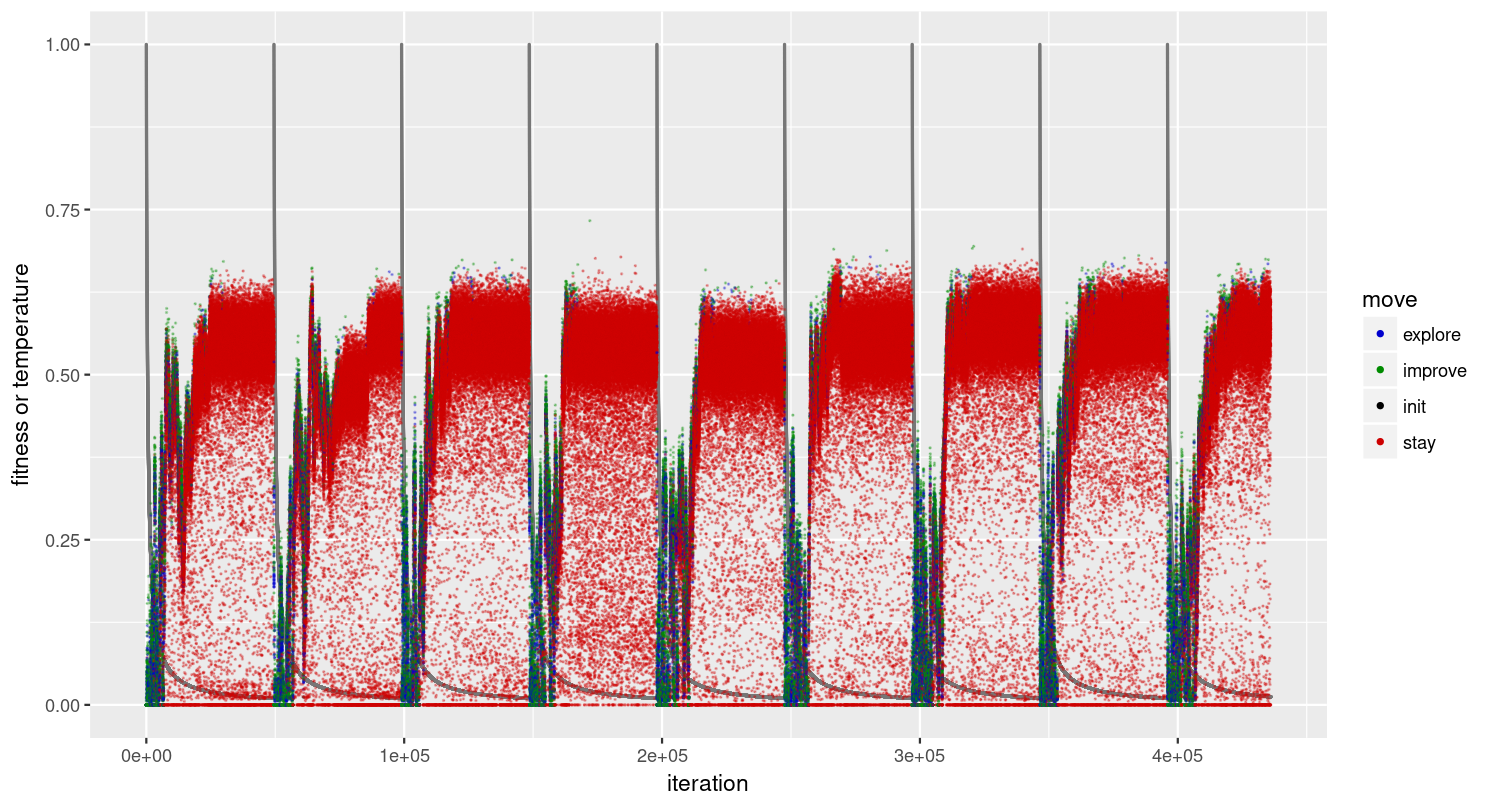
\includegraphics[width=\textwidth]{figures/sa-progress}
    \caption{The complete SA process with multiple re-annealings}
    \label{fig:sa-progress}
\end{figure}

Seen in Figure~\ref{fig:sa-progress-close} the points cluster around the same score, indicating that the locality of the grammar distribution mutations is good, or at least not bad.
A the same time there is some points spread fairly uniformly between the clustering and 0, meaning that there are some mutations that have bad locality.
Additionally there is a clustering at exactly 0, indicating a discontinuity in the fitness metric, which is most likely caused by the ``nothing'' metric that sets the score to 0 if there are no branches in the plant.
This may happen if the L-system does not contain any drawing instruction (\textit{F}), or if the number of instructions hits the maximum limit.

\begin{figure}
    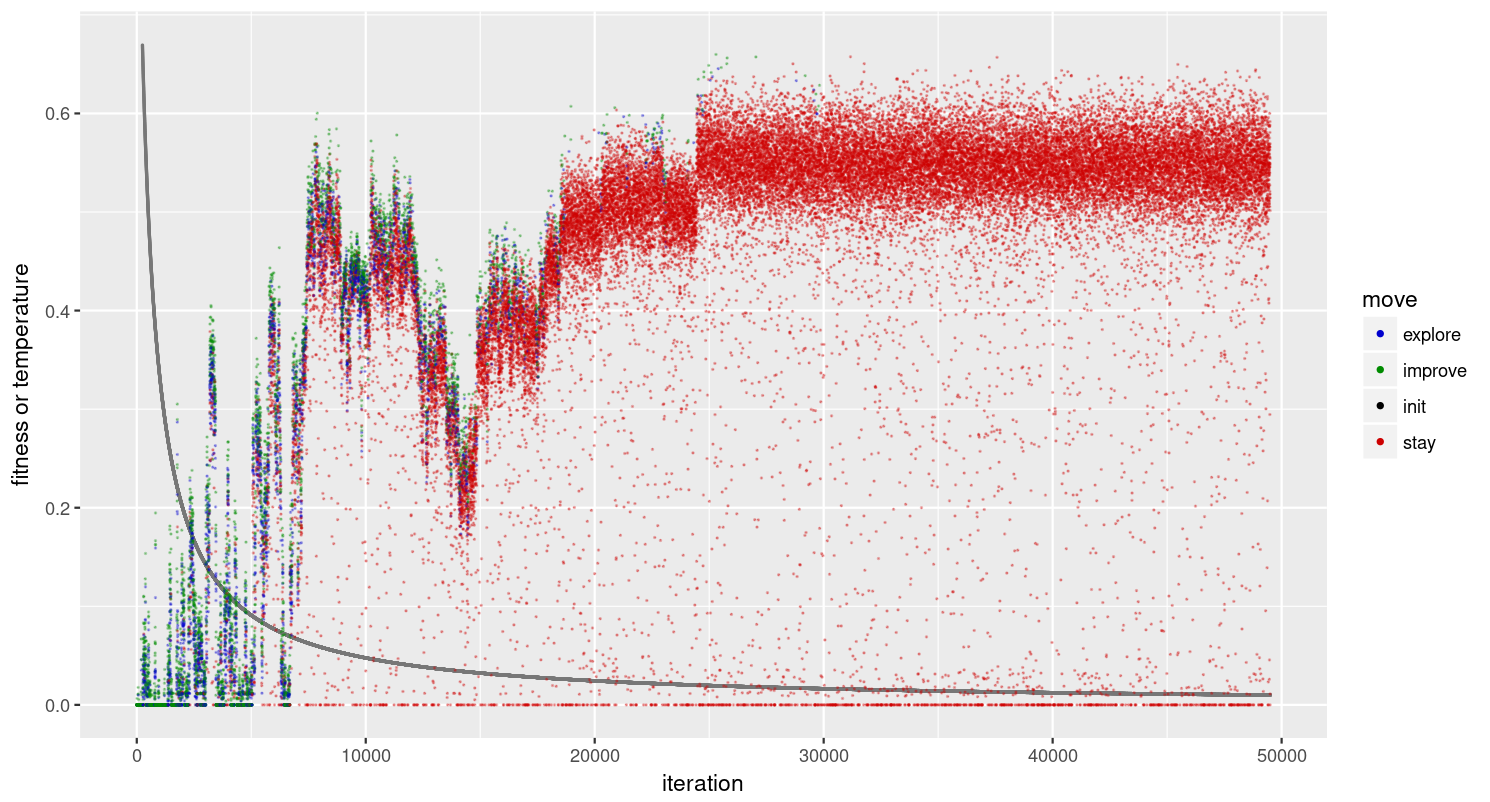
\includegraphics[width=\textwidth]{figures/sa-progress-close}
    \caption{Close-up of the first annealing of the SA process}
    \label{fig:sa-progress-close}
\end{figure}

% Is it OK to use a Mann-Whitney U test here? Are the distributions similar? Not really...
Figure~\ref{fig:sa-uniform} shows a comparison of L-system populations generated by the grammar distribution found by SA in Figure~\ref{fig:sa-progress} and a uniform grammar distribution.
The uniform grammar distribution has a mean fitness score of 0.00, while the SA-optimized grammar distribution's mean is 0.61.
A Mann–Whitney U test indicates that the groups are statistically significant different (p < 0.01).

Figure~\ref{fig:uniform-population} reflects the uniform grammar distribution's fitness score, where practically the whole population has a score of 0.
When removing all 0-scored individuals, another distribution presents itself in Figure~\ref{fig:uniform-population-no0}.
Here, a somewhat bell-shaped distribution around the score 0.5 is revealed for the remaining 121 individuals (0.121\% of the total).

Figure~\ref{fig:sa-population} shows the SA grammar distribution's distribution of fineness scores.
87.87\% of the SA sample population have a score larger than 0, compared to 0.121\% in the uniform sample population.
Thus the SA grammar distribution helps avoid most of the worst L-systems.
As the distribution is skewed to the left, the median may be a better estimate of the population average.
The SA grammar distribution has a median of 0.71, compared to 0.00 for the uniform grammar distribution.
Even with all individuals with score 0 removed, the SA grammar distribution leads with a median of 0.72 compared to 0.47, though the difference is smaller.

\begin{figure}
    \centering
    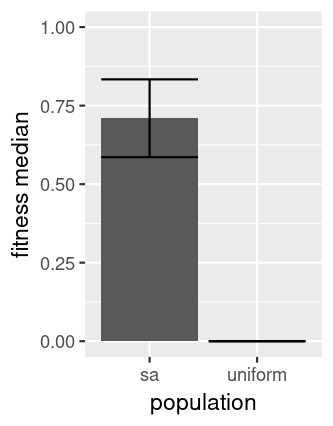
\includegraphics[width=0.4\textwidth]{figures/sa-uniform}
    \caption{Random population with uniform grammar distribution compared to SA-optimized grammar distribution}
    \label{fig:sa-uniform}
\end{figure}

\begin{figure}
    \centering
    \begin{subfigure}{0.48\textwidth}
        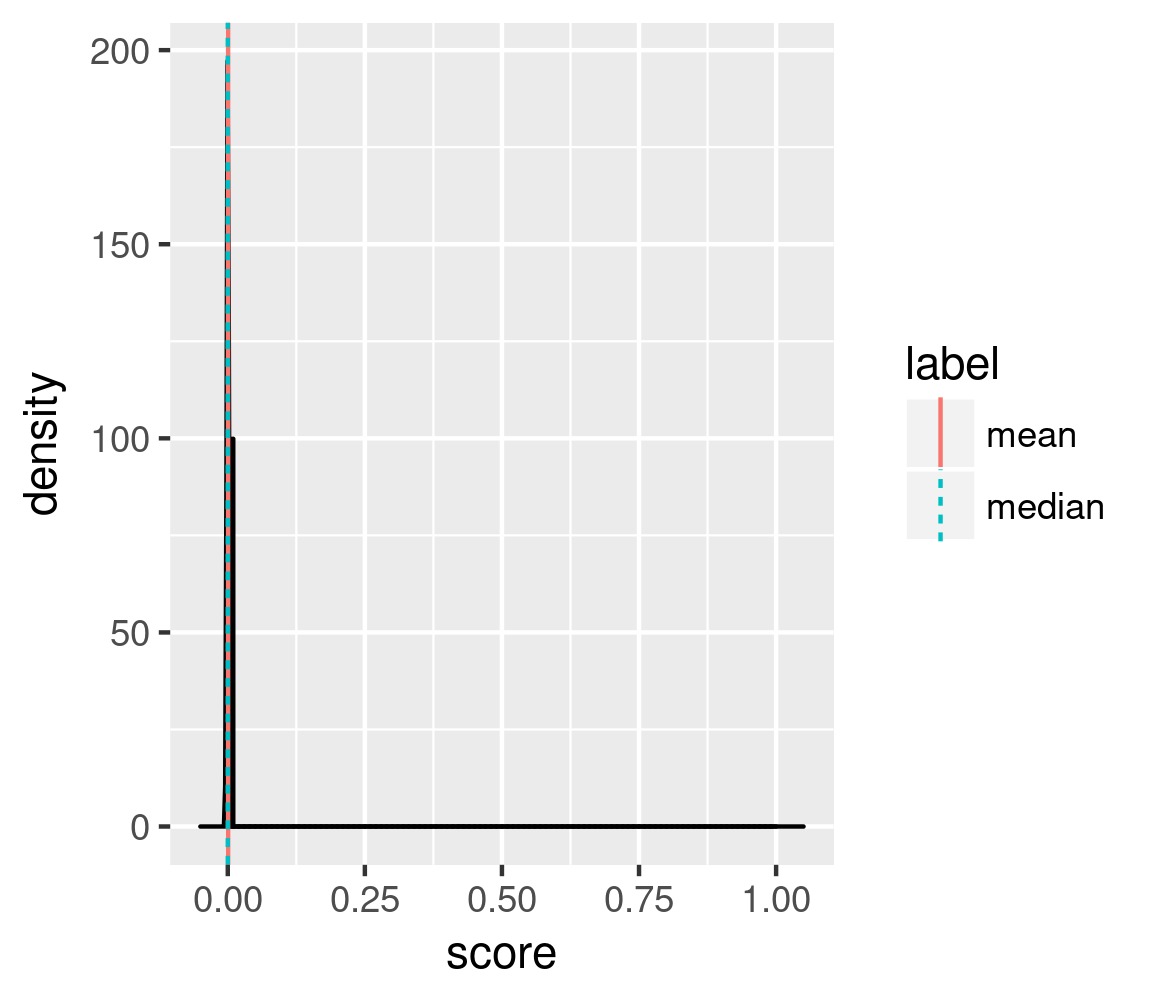
\includegraphics[width=\textwidth]{figures/uniform-population}
        \caption{Complete sample population}
        \label{fig:uniform-population}
    \end{subfigure}
    ~
    \begin{subfigure}{0.48\textwidth}
        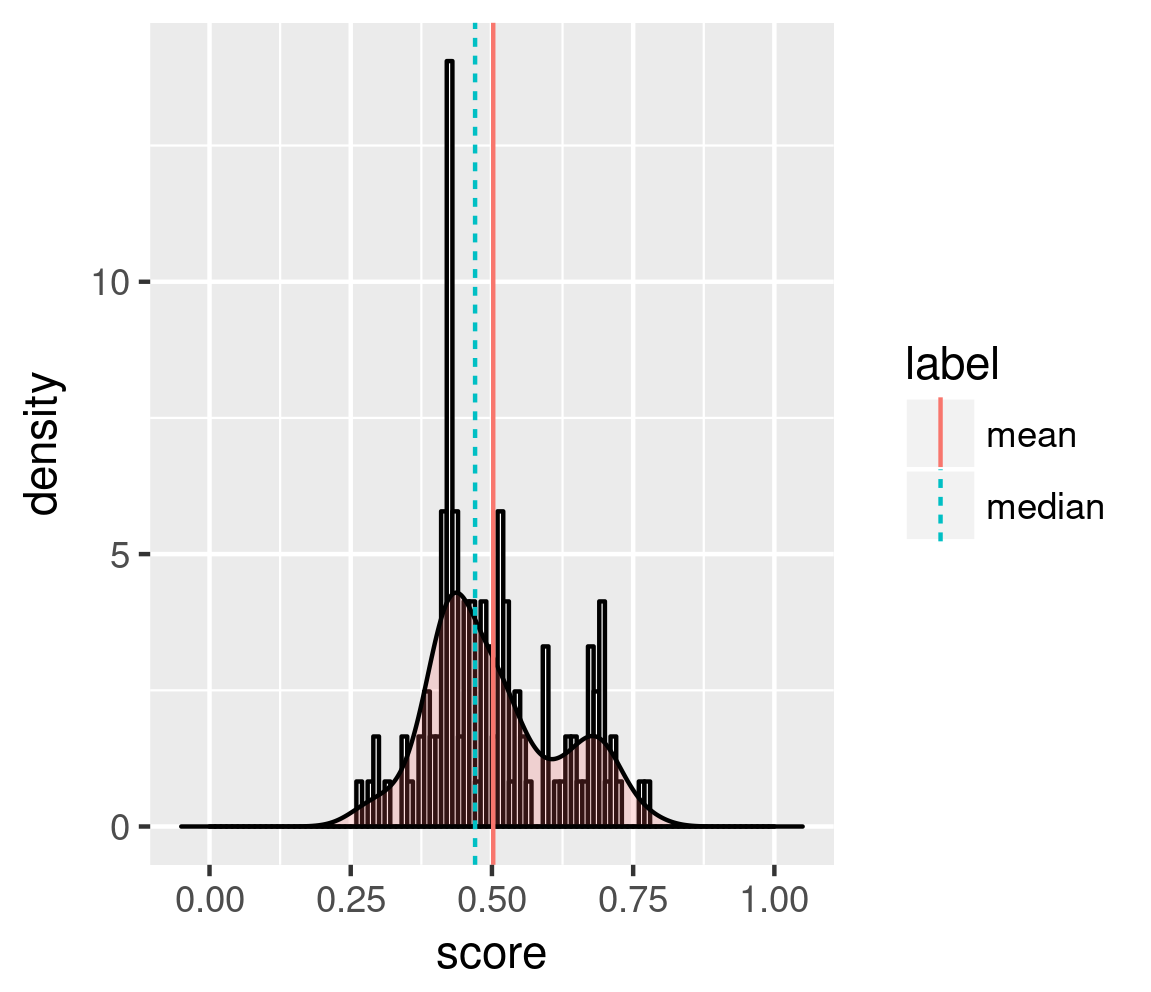
\includegraphics[width=\textwidth]{figures/uniform-population-no0}
        \caption{Sample population without samples with score 0}
        \label{fig:uniform-population-no0}
    \end{subfigure}
    \caption{Sample population of L-systems generated using a uniform grammar distribution}
\end{figure}

\begin{figure}
    \centering
    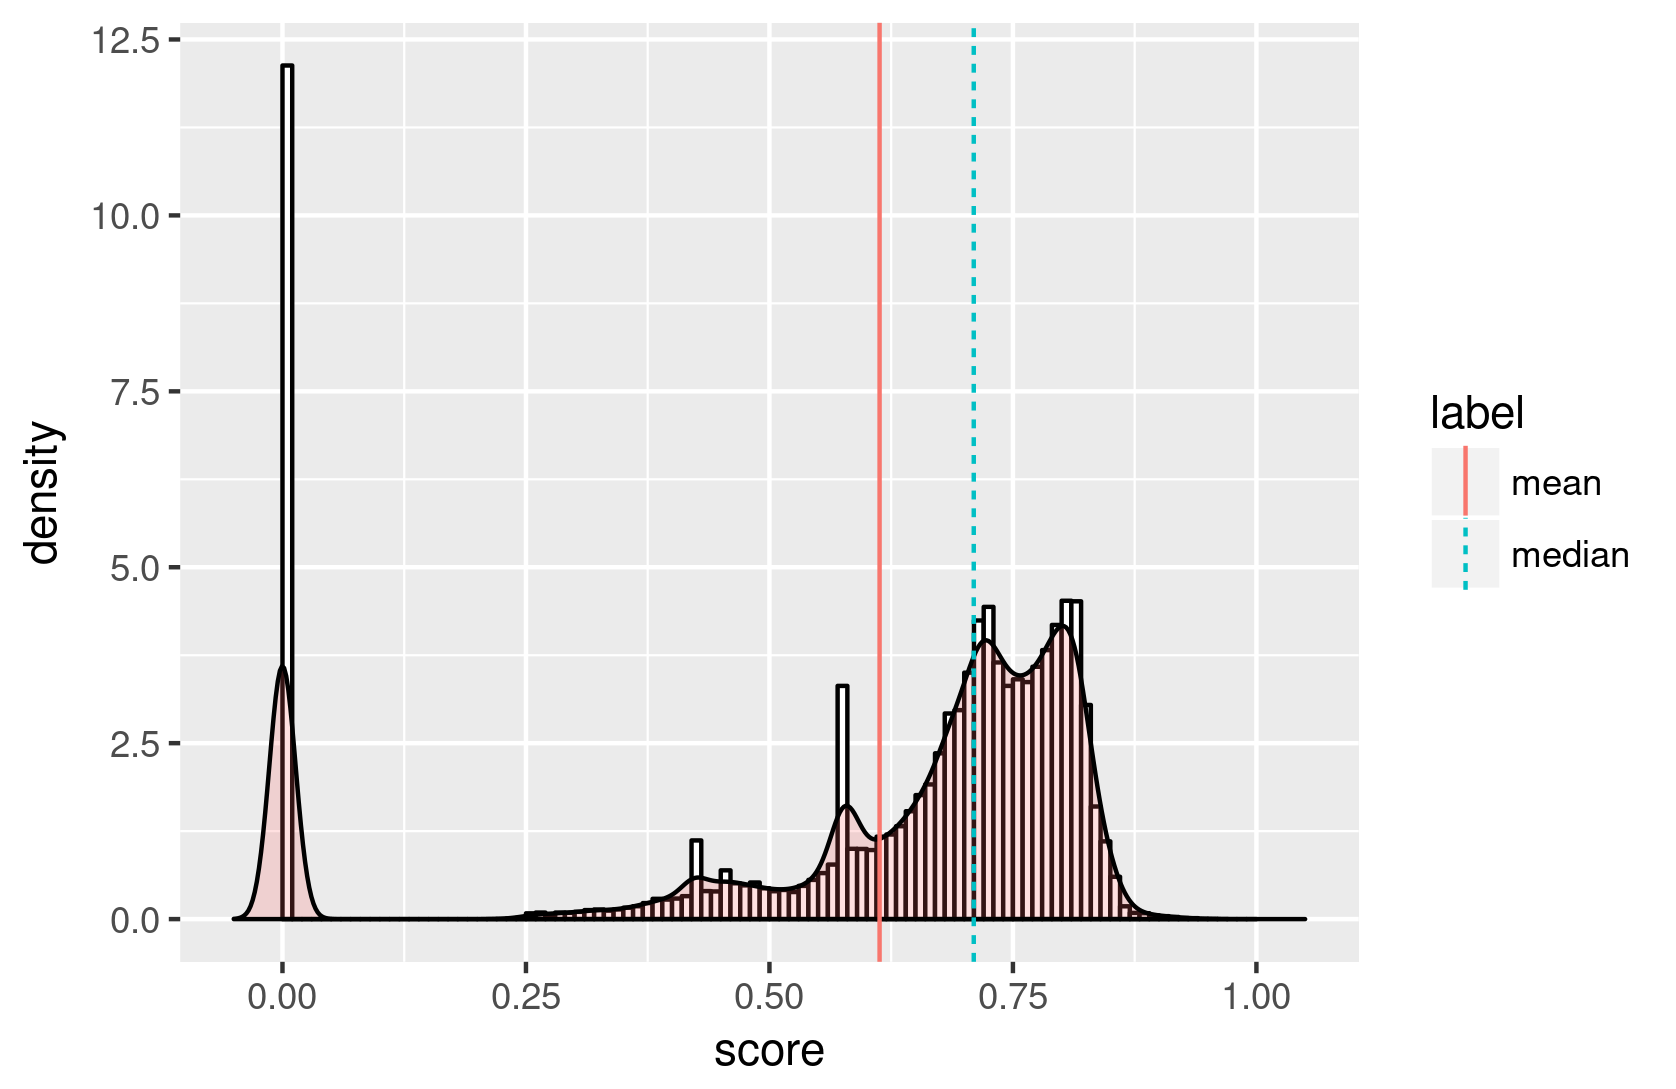
\includegraphics[width=0.8\textwidth]{figures/sa-population}
    \caption{Sample population of L-systems generated using the SA-optimized grammar distribution}
    \label{fig:sa-population}
\end{figure}

The grammar distribution found in the SA process is shown in Figure~\ref{fig:sa-dist}.
As seen in Figure~\ref{fig:sa-dist-prod}, this grammar distribution favors around 10 production rules in the L-system, though 20 productions is also a strong contender.
Figure~\ref{fig:sa-dist-stack} shows that it always favors symbols over stacks, starting at around 60\% symbols in the top depth, then around 90\% symbols in the next depth, and 100\% symbols in the final depth.
% PROBABLY CAUSED BY THE INSTRUCTION LIMIT, WHICH IS A LIMITATION.
This indicates that restricting the number of depths to 4 was not too restricting as it chose to restrict itself to 3 depths.
Additionally, this makes all of the distributions at depth 3 irrelevant as they will never be used.
It favors shorter strings in depth 0, but not too short strings, as seen in Figure~\ref{fig:sa-dist-strlen}.
% WHY NOT MEDIUM STRING LENGTHS? WHY A VALLEY BETWEEN THESE?
While in depth 1 and 2 it favors medium short and medium long strings.

Figure~\ref{fig:sa-dist-sym} shows that it only allows variables in depth 0, while its nearly the inverse in depth 1 and 2.
This is interesting as an operation has no effect if it is not followed by a variable.
Thus depth 2, along with depth 3, is not contributing anything to the plant, but depth 2 is still wasting instructions.
Depth 1 also has only about 10\% chance of a variable, meaning that most of the drawing will happen in depth 0, which in turn means less branching.
% THE ABOVE CAN BE SEEN IN THE PLANTS GENERATED FROM THIS DISTRIBUTION.

The operation distribution in Figure~\ref{fig:sa-dist-op} is difficult to understand, but the strong "-" in depth 0 should make the branches have a tendency to bend towards one side.
Among all of the 20 variables available, \textit{F} is the only variable that is an instruction, the draw line instruction.
As expected, Figure~\ref{fig:sa-dist-var} shows that it is included and is one of the stronger variables in the distribution.
Without the \textit{F} variable, the L-systems would have no branches and thus get score 0.
Only 3--4 of the variables have a strong weight in each of the depths, indicating that it understands that focusing on a fewer set of variables may lead to less ``nothing'' plants.

% might split these into separate figures and put them inbetween the above paragraphs
\begin{figure}
    \centering
    \begin{subfigure}{0.48\textwidth}
        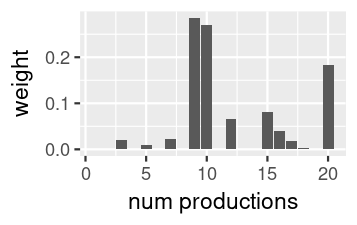
\includegraphics[width=\textwidth]{figures/sa-dist-prod}
        \caption{1*20production}
        \label{fig:sa-dist-prod}
    \end{subfigure}
    ~
    \begin{subfigure}{0.48\textwidth}
        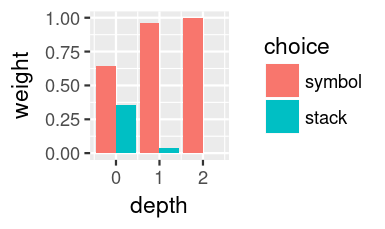
\includegraphics[width=\textwidth]{figures/sa-dist-stack}
        \caption{symbol / stack}
        \label{fig:sa-dist-stack}
    \end{subfigure}
    \\
    \begin{subfigure}{0.98\textwidth}
        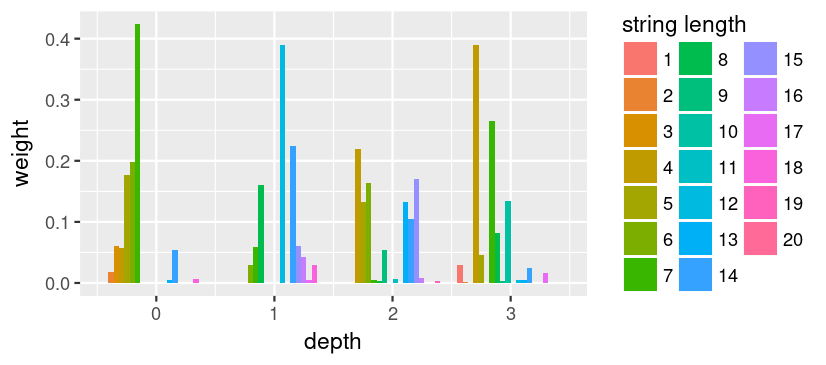
\includegraphics[width=\textwidth]{figures/sa-dist-strlen}
        \caption{1*20(symbol / stack)}
        \label{fig:sa-dist-strlen}
    \end{subfigure}
    \\
    \begin{subfigure}{0.4\textwidth}
        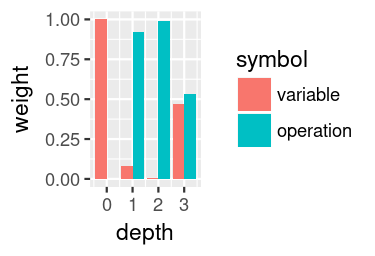
\includegraphics[width=\textwidth]{figures/sa-dist-sym}
        \caption{variable / operation}
        \label{fig:sa-dist-sym}
    \end{subfigure}
    ~
    \begin{subfigure}{0.57\textwidth}
        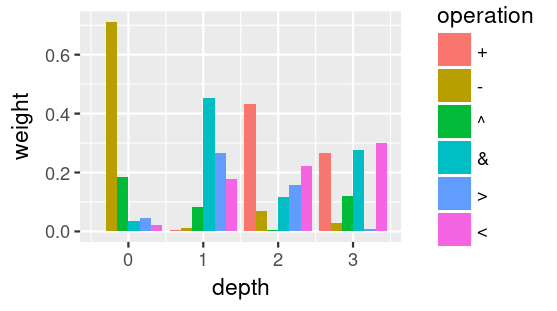
\includegraphics[width=\textwidth]{figures/sa-dist-op}
        \caption{"+" / "-" / "\textasciicircum" / "\&" / ">" / "<"}
        \label{fig:sa-dist-op}
    \end{subfigure}
\end{figure}
\begin{figure}
    \ContinuedFloat
    \begin{subfigure}{0.98\textwidth}
        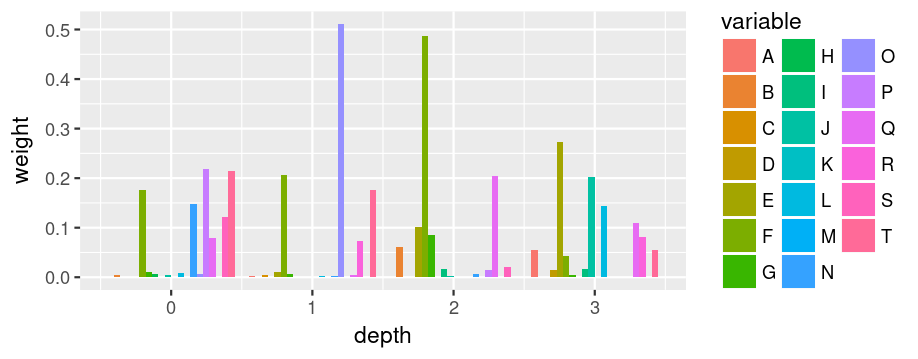
\includegraphics[width=\textwidth]{figures/sa-dist-var}
        \caption{\%x41-55}
        \label{fig:sa-dist-var}
    \end{subfigure}
    \caption[SA-optimized grammar distribution]{SA-optimized grammar distribution. Captions are the respective parts of Listing~\ref{lst:grammar}.}
    \label{fig:sa-dist}
\end{figure}

% Try to connect this to the above even more.
The above analysis of the grammar distribution is reflected in the produced L-system and 3D plant models.
An example of a generated plant can be seen in Figure~\ref{fig:sa-plant}, and its L-system in Listing~\ref{lst:sa-plant}.
This plant is very tall and straight, has few branches and few fractal patterns.
All of this is likely caused by the depth 3 not being relevant, depth 2 being practically not relevant, and depth 1 being nearly not relevant.
The L-system goes to depth 2, but depth 2 never includes any symbols, thus not being relevant.
Depth 1 is mostly producing operatiors, but also an occational variable, thus being useful and producing the lateral branches seen on the plant.
There is recursion in the segment drawing as \textit{F} produces \textit{P} and \textit{T} which in turn produce \textit{F}.
Additionally, part of the recursion is inside a stack, thus allowing for fractal patterns.

\begin{figure}
    \centering
    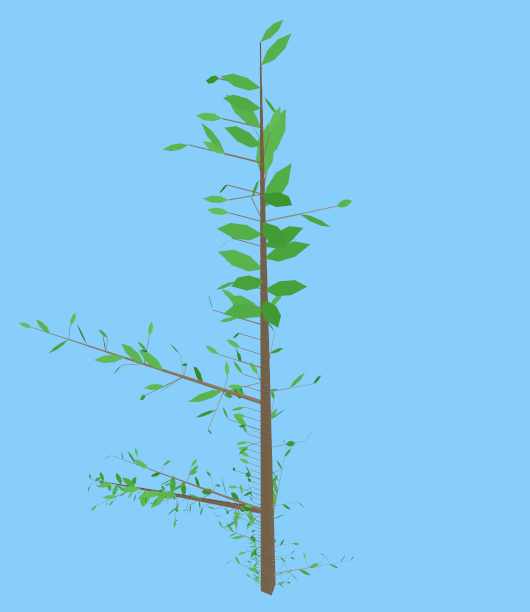
\includegraphics[width=0.6\textwidth]{figures/sa-plant}
    \caption[Example plant generated by the SA-optimized grammar distribution]{Example plant generated by the SA-optimized grammar distribution, fitness 0.78}
    \label{fig:sa-plant}
\end{figure}

\begin{lstlisting}[caption=L-system representation of plant in Figure~\ref{fig:sa-plant}, label=lst:sa-plant, float]
axiom: NT[>>&&&&>&&&F[++++<<]]P[<<&^[>-+<+>]&><&&&&&O]P
F -> Q[O&^&&&^&<>O[<<+++++^>++<++&][++++-]&>]NT[^>R>&>[<<&<+&+&<+&+-<]<<>&&]P
L -> [O&<<>&^&&&&>]S[^<[+++-<<>>++<<+<-]^>&<<&>&&>F^>]T[<<&><^&&O&<>]
N -> N[><&<^&<<&&^&&T][&>[+-<<>+++&+&<+][+++++&><++><<^-]&&&>]PN[&&>&>T&&&&^&><<&]
P -> [&&&O>&>&&>>&&F]F[<&&&&&&>&&&&]TF
S -> [><&<&&>&]TSQS[&T<<<>[>++-+]<<&&>]T
T -> PT[>&^>&&&>&&R&&<>>]
\end{lstlisting}

\section{Evaluation of Evaluation Module}
\subsection{Method}
\textbf{RQ2} asks ``how aesthetically pleasing plants can be generated''.
DGEL was the developed solution to this question, but to know if it can actually generate aesthetically pleasing plants or not, the evaluation module has to be analyzed and compared to how humans rank the plants.
If the ranking made by the humans agree with the ranking made by the fitness component in the evaluation module, it would mean that the generator know how to distinguish good plants from bad plants, and can thus apply its evolutionary algorithms to generate aesthetically pleasing plants.
Thus the hypothesis is: Humans agree with the ranking made by the DGEL fitness component.

Both a quantitative method and a qualitative method will be used for this purpose.
The quantitative method aims to answer if the humans agree with the DGEL ranking.
If they do not completely agree, the qualitative method will be used to analyze why they do not agree and what the important features of a plant that makes it aesthetically pleasing are.

A pairwise comparison of a set of DGEL-generated plants will be performed by human participants.
The analytical hierarchy process (AHP) will be used to take the pairwise comparison data for a participant and create a ranking of all of the plants~\cite{2008Saaty}.
% Write about AHP, and why I used it?
Finally, all of the rankings will be aggregated and compared to the ranking made by DGEL using Kendall's Tau~\cite{1938Kendall}, and dRank~\cite{2009Carterette}.
Kendall's Tau will test the ranking correlation and its requirement of the rankings fit the requirements of Kendall's Tau~\cite{2010Webber}: they are unweighted, conjoint and have a definite range.
It will also give an indication of how correlated they are in range $[-1, 1]$, where 1 is perfectly positively correlated, 0 is not correlated and -1 is perfectly negatively correlated.
But there are two problems with it: it does not consider the relative distances between the ranks~\cite{2010Webber}, and the different participant's rankings will have to be aggregated beforehand, meaning Kendall's Tau does not consider the variance between these rankings.
Thus, dRank will be used as an alternative statistic, as it considers the distances between ranks and that there are multiple rankings aggregated together~\cite{2010Webber,2009Carterette}.

As many plants as possible were desired, but humans have a limited patience and the number of comparisons to rate is $\frac{n * (n - 1)}{2}$, where $n$ is the number of plants.
Thus a limited set of plants had to be used.
The final number of plants used is based on the estimated time used on a comparison and the estimated time a participant is patient.
The plants should also be spread over the range of the fitness score, so that the rank comparison will be valid for the complete range.
They should also always be \textit{something} (have at least one branch), otherwise there is nothing to rate.
The ideal score range would be $[0, 1]$, but it was found difficult to generate plants perfect 0 (with the plant being \textit{something}) and 1 scores.
Thus GE was used to generate the worst possible plant with score above 0, and the best possible plant.
Then, $n - 2$ plants were generated uniformly between these two extremes.

% Actually, I was the very first pilot run.

To find a good estimate for the number of plants, and to test the quality of the overall survey, two pilot runs were performed.
The first pilot run was based on an estimate made by the researcher's own experience in taking the survey.
One participant participated and was observed through the whole survey.
They were asked to complete the survey as described in it, think aloud, tell us when they get tired and answer some questions at the end.
% Exactly which questions?
Based on this, the amount of plants were changed, the fitness metric was modified, and the overall survey was improved.
The second pilot run were with the same participant, where they were asked to retake the survey and provide feedback on the changes.
Based on this feedback, the final survey was formed.

Participants were sampled using convenience sampling and snowball sampling.
As such, the results may not be generalizable to the whole population, but they may be used as an indication to what is important in an aesthetically pleasing plant.
Convenience sampling was selected because of time and resource restrictions.
In addition, snowball sampling was added as a means to gather more samples.
Participants were found by asking friends, family and acquaintances either by direct conversation or by posting publicly on social networks including Facebook, Google+ and Twitter.
The participants were asked to share the survey to others, and a sharing link was shown at the end of the survey, thus allowing for a snowballing effect.

% plants are video recordings
% four observations

\subsection{Survey Design}
% link to consent?
% link to survey?
The survey consists of a consent that they need to agree with, a pre-questionnaire, a description, the pairwise comparison, a post-questionnaire with the results, and finally a thank-you page with the sharing link.
The pre-questionnaire is intended to map the demographic and what relation they have to plants and games.
The description describes the pairwise comparison task, what they should do in it, and what to expect at the end.
The post-questionnaire is intended to find how much the participant agree with the ranking calculated by AHP or why they do not agree, and what they find important in plants.
Finally, the thank-you page is used to assure the participant that they have completed the survey, give them the option to see or share their results, and share the survey to others.

In the pre-questionnaire the participants are first asked about their age, gender, education and occupation.
They are then asked ``how often do you work with plants?'' and ``how much do you like plants in general?''
Their purpose is to see if their relation to plants affects how they rank the plants.
Finally, they are asked ``how often do you play video games?''
This is to see if their relation to video games affects how they rank the plants.
A person that regularly works with plants or enjoys looking at plants in nature may expect something different in a plant than a person who regularly see plants in video games.

During the description of the task, they are recommended to enter fullscreen such that they do not have distractions and that the plants can be viewed as big as possible.
They are also asked to try a different browser or withdraw if the plant visualization is not working as expected.
This is because the quality of the visualization may affect their ratings.

\begin{figure}
    \centering
    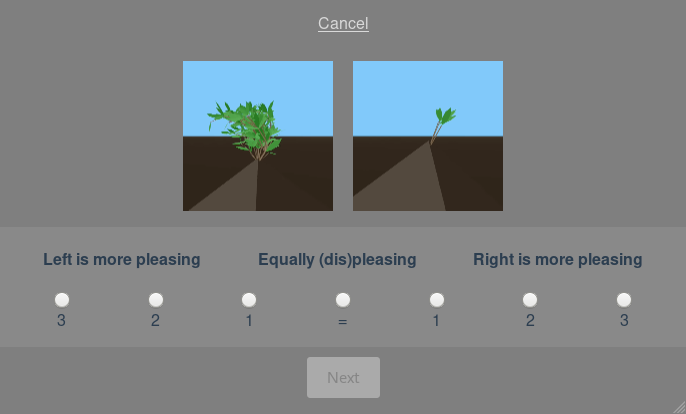
\includegraphics[width=1.0\textwidth]{figures/pairwise}
    \caption{Pairwise comparison task as viewed on a small screen}
    \label{fig:pairwise}
\end{figure}

Figure~\ref{fig:pairwise} shows the comparison task.
It is kept as simple as possible to avoid distractions, and a neutral gray background color is used to avoid the percieved hue or brightness of the plants to be shifted.
Two plants are visualized side by side as looping videos of a camera rotating around the plant such that all sides of the plant is seen.
In addition, the camera adjusts its height and distance from the plant so that all of the plant can be viewed.
The rotation happens at a balanced speed that lets the user view all of the plant in a short amount of time, while being slow enough to let them study it.
% The pilot confirmed that the speed was good.
The video runs at 60 frames per second (FPS) to give a smooth experience, to match the monitor refresh rate and to match what is commonly used in games.

The participant is presented with three categories to choose between: left is more pleasing, they are equally (dis)pleasing, and right is more pleasing.
If they find one more pleasing they need to rate how much pleasing it is on a scale of 1 to 3.
The original AHP method uses a 8-point scale, but this is too detailed for a ``normal human'', and thus it was reduced to 3 points which allows for a low, medium and high rating.
Based on feedback from the pilot run, the ``equally (dis)pleasing'' option was labeled \textit{=} instead of 0 because 0 seemed like it meant that the plants were bad.
``(dis)'' was also added based on the feedback because without it it seemed like it meant that the plants were good.
With the changes, the participant should be less reluctant to select ``equal''.

By pressing the ``next'' button, the participant will be presented with new pairs until all have been rated.
The pairs are presented in random order and with random placement (left or right), as to not make the order create a bias.

\begin{figure}
    \centering
    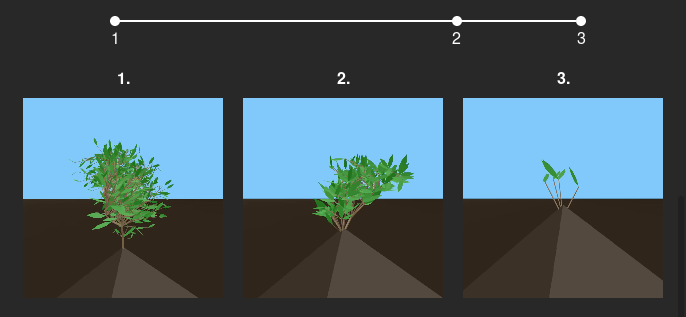
\includegraphics[width=1.0\textwidth]{figures/rank}
    \caption{Example rank resulting from human rating of plant pairs}
    \label{fig:rank}
\end{figure}

The post-questionnaire asks some questions and displays the resulting order of the plants.
Figure~\ref{fig:rank} shows an example of the resulting order.
The dots on the white line represents the relative distance between the plants, and the plants them selves are shown in order below.
% Explain how this is done.
In this example, the plant ranked as the best is much more better than the second than the second is to the third.
The participants are asked if they ``agree with the ranking of the plants shown below'', and if they do not strongly agree, they are asked ``why do you not strongly agree with the ranking?''
This can help determine if the method of ranking the plants with AHP is valid.
Next they are asked the most important question: ``What would you say separates good plants from bad plants in the ranking?''
This is useful to be able to do a qualitative analysis of why the human ranking does not match the fitness ranking, if they do not match.
Finally, they are asked for ``other comments'' in case they have something useful to add that do not fit the other questions.

The final thank-you page contains a congratulation, a link to revisit their results, and a link to share the survey.
This share link contains a token that indicates who it was shared from.
With this data the snowball effect can be tracked.
Though, there is nothing preventing them from sharing the original link, thus losing this information.

\subsection{Implementation}
No web-based application the matches the design of the survey was found.
Thus as single-page web-application was created using the Vue JavaScript framework for in the front end, the Rocket web framework for Rust in the back end, and MongoDB to store the data.
Multiple other libraries were used both in the front end and back end, but the aforementioned are the most central.
As the application is a on-off application, only meant to be used for the survey, and fairly simple, the choices of technology and architecture were based on experience, convenience and preferences.
Most of the technology used had recently been used in another project by the researcher, and thus allowed for code re-use and rapid development.

The application uses a client--server architecture, as shown in Figure~\ref{fig:pairwise-architecture}, where the server consists of two layers: API and DB.
The client uses a Vue Component for each page described in the Survey Design, and URL routing is handled by Vue Router.
The Components communicated directly to the API layer using a custom REST API, to for example register a participant or get the pairs of plants to evaluate.

The API layer is written in Rust and uses the Rocket framework to implement the API.
Multiple routes are defined based on the requirements of the client.
It communicates directly to the MongoDB database using the \textit{mongodb} Rust library.

When a participant registers, they receive a private token that is kept in the URL in the client throughout the whole survey.
This token access to submit and retrieve their data.
They also receive a public token that represents the participant, but does not grant access to their data.
Thus, this public token is used in the share link to identify who shared it.

The paricipant participates only in a specific \textit{task}.
A task is a set of plants that are to be evaluated, and the system may contain multiple tasks.
While only one task is used during the survey, allowing multiple tasks lets the researcher experiment with the application without affecting the real data while developing or during the survey.

The database contains three collections: \textit{user}, \textit{sample} and \textit{weight}.
\textit{user} stores all data relating to the user and is uniquely identified by the private and public tokens individually.
\textit{sample} stores data about one of the plants, such as its name and the task it is part of.
Finally, \textit{weight} stores the rating submitted by one user for one pair of plants and is uniquely identified by the user and the two plants together.

Finally there is a command-line interface (CLI) available to extract the data either as raw data or as calculated priority weights using AHP.
Because of this, a separate module \textit{stats} in the API layer containe the common functionality used by both the API and the CLI.

\subsection{Results}
% BAAAAAAAAH
